%----------------------------------------------------------------------------------------
%	PACKAGES AND OTHER DOCUMENT CONFIGURATIONS
%----------------------------------------------------------------------------------------

\documentclass[final,hyperref={pdfpagelabels=false}]{beamer}

\usepackage[orientation=portrait,size=a0,scale=1.4]{beamerposter} % Use the beamerposter package for laying out the poster with a portrait orientation and an a0 paper size

% \toprule, \midrule, \bottomrule % instead of \hline
\usepackage{booktabs}
% Tables that can fit page length
\usepackage{tabularx}
% Multirows and multicolumns in table
\usepackage{multirow, multicol}

\usetheme{I6pd2} % Use the I6pd2 theme supplied with this template
\usepackage[english]{babel} % English language/hyphenation
\usepackage{amsmath,amsthm,amssymb,latexsym} % For including math equations, theorems, symbols, etc

%\usepackage{times}\usefonttheme{professionalfonts}  % Uncomment to use Times as the main font
%\usefonttheme[onlymath]{serif} % Uncomment to use a Serif font within math environments

%\boldmath % Use bold for everything within the math environment

\graphicspath{{media/}} % Location of the graphics files
\usecaptiontemplate{\small\structure{\insertcaptionname~\insertcaptionnumber:\,}\insertcaption} % A fix for figure numbering
\usepackage{siunitx}
\usepackage{caption}

%set reference on one line
\setbeamertemplate{bibliography entry article}{}
\setbeamertemplate{bibliography entry title}{}
\setbeamertemplate{bibliography entry location}{}
\setbeamertemplate{bibliography entry note}{}


% Acronyms
\usepackage{acronym}
\acrodef{SLAM}{simultaneous localization and mapping}
\acrodef{SOTA}{state-of-the-art}
\acrodef{SSMR}{skid-steering mobile robot}
\acrodef{AMR}{Ackermann mobile robot}
\acrodef{UGV}{Uncrewed ground vehicle} %FP: more gender neutral
\acrodef{IDD}{ideal differential-drive}
\acrodef{ICR}{instantaneous center or rotation}
\acrodef{RTK}{Realtime Kinematics}
\acrodef{GNSS}{Global Navigation Satellite System}
\acrodef{ROC}{radius of curvature}
\acrodef{IMU}{inertial measurement unit}
\acrodef{MPC}{model predictive control}
\acrodef{GP}{Gaussian processe}
\acrodef{BLR}{Bayesian Linear Regression}
\acrodef{IPEM}{integrated prediction error minimization}
\acrodef{MLP}{multilayer perceptron}
\acrodef{ICP}{iterative closest point}
\acrodef{MRMSE}{multi-step root mean squared error}
\acrodef{T-MRMSE}{translational multi-step root mean squared error}
\acrodef{R-MRMSE}{rotational multi-step root mean squared error}
\acrodef{M-Z-score}{multi-step Z-score}
\acrodef{DRIVE}{Data-driven Robot Input Vector Exploration}
\acrodef{VISTA}{Vehicle Input Space Training Assistant}

% models
% \bm % in equations for proper bold font
\usepackage{bm}
\newcommand{\DOUGHNUTCALIB}{\ac{DRIVE}\xspace}
\newcommand{\ICRBASED}{\ac{ICR}-based\xspace} 
\newcommand{\DIMPARAMS}{\bm k}
\newcommand{\HORDUR}{h_d}
\newcommand{\WINSIZE}{h}
\newcommand{\TRAINDATA}{$\mathcal{D}$\xspace}
\newcommand{\DOUGHNUTDATA}{$\mathcal{D}_D$}
\newcommand{\HUMANDATA}{$\mathcal{D}_H$}
\newcommand{\PREDSTATE}{\,^\mapf\!\hat{\bm q}}
\newcommand{\MEASSTATE}{\,^\mapf\bm q}
\newcommand{\MARMOTTE}{HD2\xspace}
\newcommand{\CMDBODYVEL}{^{\robotf}\bm{f}}
\newcommand{\SLIPBODYVEL}{^{\robotf}\bm{g}}
\newcommand{\OBSERVEDSLIP}{\bm{g}}
\newcommand{\INPUTVECTOR}{\bm{u}}
\newcommand{\STATEPROPMAT}{_{\robotf}^{\mapf}\bm{T}\left(^\mapf\theta_t\right)}
\newcommand{\INPUTSPACE}{\mathcal{J}}
\newcommand{\BODYVELSPACE}{\mathcal{B}}
\newcommand{\CENTRIFUGAL}{\psi}
\newcommand{\OPTIMCALIBTIME}{$t_{\text{opt}}$\xspace}
\newcommand{\robotstate}{\bm{q}}
\newcommand{\mapf}{\mathcal{G}} % map reference frame
\newcommand{\robotf}{\mathcal{R}} % robot reference frame
\newcommand{\learnedslip}{\bm{\Xi}}
\newcommand{\blrweights}{\bm{\gamma}}
\newcommand{\blrinputs}{^{\robotf}\bm{x}}
\newcommand{\MRSME}{\epsilon}

%----------------------------------------------------------------------------------------
%	TITLE SECTION 
%----------------------------------------------------------------------------------------

\title{\huge DRIVE: Data-driven Robot Input Vector Exploration} % Poster title

\author{\normalsize Dominic Baril$^{1}$, Simon-Pierre Deschênes$^{1}$, Luc Coupal$^{1}$, Cyril Goffin$^{2}$, \\Julien Lépine$^{1}$, Philippe Giguère$^{1}$, François Pomerleau$^{1}$} % Author(s)} % Author(s)

\institute{\small$^1$ Northern Robotics Laboratory, Universit\'e Laval \small$^2$ École Polytechnique Fédérale de Lausanne} % Institution(s)

%----------------------------------------------------------------------------------------
%	FOOTER TEXT
%----------------------------------------------------------------------------------------

\newcommand{\leftfoot}{IEEE International Conference on Robotics and Automation 2024} % Left footer text

\newcommand{\rightfoot}{\{dominic.baril, francois.pomerleau\}@norlab.ulaval.ca} % Right footer text

%----------------------------------------------------------------------------------------

\begin{document}

\addtobeamertemplate{block end}{}{\vspace*{1ex}} % White space under blocks

\begin{frame}[t] % The whole poster is enclosed in one beamer frame

\begin{columns}[t] % The whole poster consists of two major columns, each of which can be subdivided further with another \begin{columns} block - the [t] argument aligns each column's content to the top

\begin{column}{.0125\textwidth}\end{column} % Empty spacer column

\begin{column}{.465\textwidth} % The first column

%----------------------------------------------------------------------------------------
%	OBJECTIVES
%----------------------------------------------------------------------------------------
\vspace{-12.5mm}
\begin{block}{Context \& Motivations}
\begin{itemize}
	\item A motion model is a key component of autonomous navigation systems, but \acp{UGV} behavior varies significantly depending on terrain and vehicle properties.
	\item Sensory measurements and information on ground properties are limited.
	\item Empirical training dataset gathering is energy and time consuming~\cite{Williams2018}, two critical resources for remote deployments.
	\item Facilitating and automating the task of gathering a training dataset if of high importance for field operations.
\end{itemize}
\end{block}

\begin{block}{\acf{DRIVE}}
	\begin{figure}
		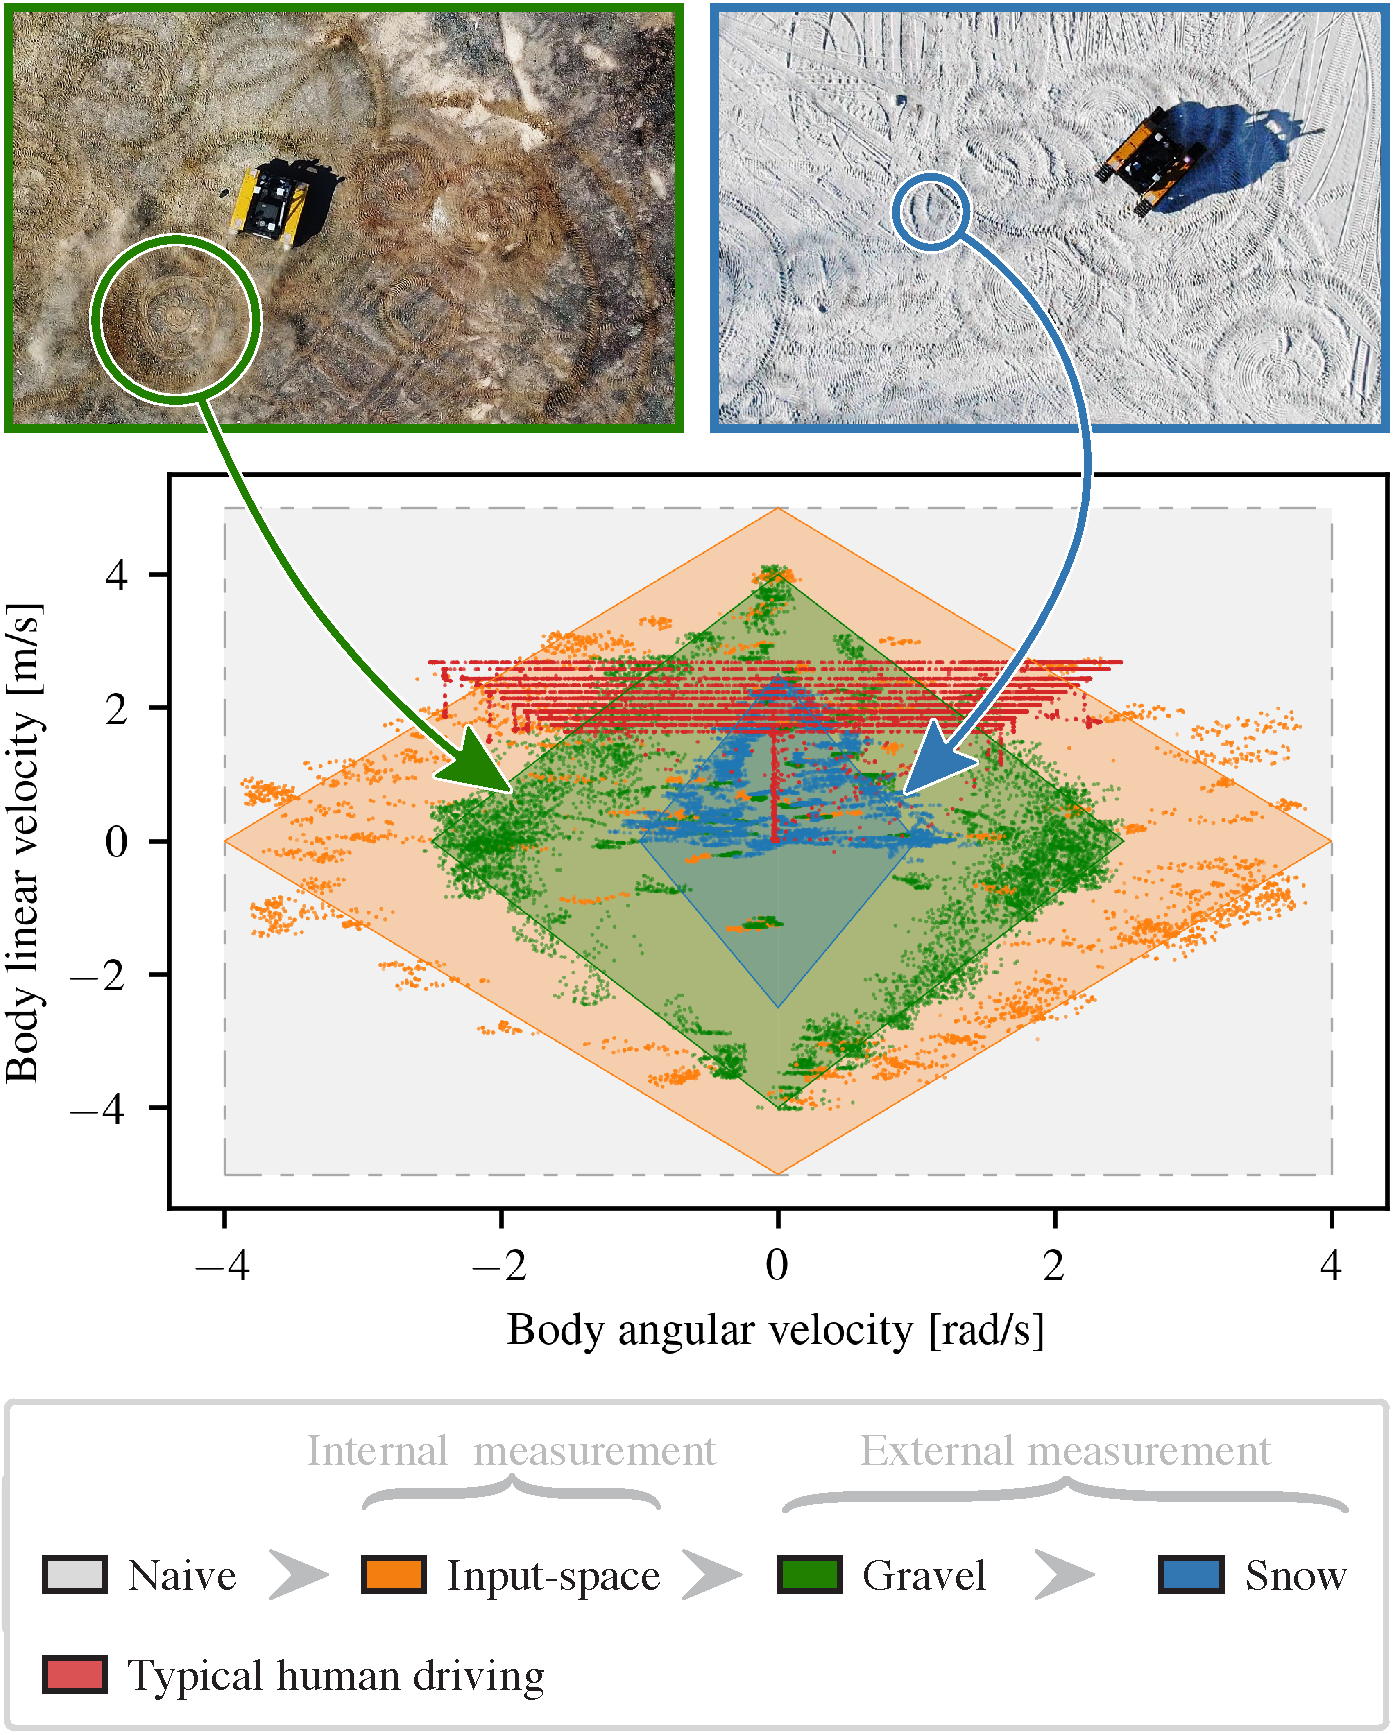
\includegraphics[width=0.785\linewidth]{figures/Figure_1_final_no_margin.pdf}%
		%\vspace{-7mm}
		\captionsetup{width = 0.975\linewidth, justification=justified, name=Figure 1}
		\caption{
			Vehicle and terrain characterization done through DRIVE.
			The manufacturer-defined Naive input-space region is drawn in gray.
			The vehicle's true input-space, characterized through internal measurements, is shown in orange.
			Typical human driving is shown in red.
			% The scatter dots show the uniform input-space sampling in orange and resulting body velocities estimated through external measurements in green and blue.
			The resulting body velocities are represented in green for gravel and blue for snow.
			%The resulting terrain-dependent body velocity is shown as the green diamond for gravel and blue diamond for snow.
			% We observe a~\SI{50}{\%} area reduction between naive and true input-space, then another~\SI{50}{\%} area reduction between external calibration and internal calibration.
			% The equivalent internal to external reduction is of~\SI{87.5}{\%} for snow.
		}
		\label{fig:simu}
	\end{figure}
		\begin{itemize}
		\item Automated protocol for input space characterization and dataset gathering.
		\item Random uniform input sampling minimized input bias and stimulates dynamic, transitory behavior.
		\item Improvement in prediction accuracy of~\SI{31.8}{\%} in translation and~\SI{43.6}{\%} in rotation over angular-focused and linear-focused methods respectively. 
		\item \SI{6}{\second} intervals to stimulate transitory and steady behavior.
		\item Driving time of~\SI{46}{\second} required to train a motion model.
	\end{itemize}
	\begin{table}[!ht]
		\caption{
			Median prediction improvement for all robots and terrains.
		}
		\label{tab:drive_improvement}
		\centering
		\small
		\begin{tabularx}{0.9\textwidth}{l*{6}{>{\centering\arraybackslash}X}}
			\toprule
			Prediction & \multicolumn{2}{>{\hsize=\dimexpr2\hsize+2\tabcolsep+\arrayrulewidth\relax}c}{Husky}
			& \multicolumn{2}{>{\hsize=\dimexpr2\hsize+2\tabcolsep+\arrayrulewidth\relax}c}{HD2}
			& \multicolumn{2}{>{\hsize=\dimexpr2\hsize+2\tabcolsep+\arrayrulewidth\relax}c}{Warthog} \\
			improvement & Tile & Snow & Tile & Snow & Gravel & Ice \\ \toprule
			Translation (\%) & 35 & 10 & 33 & 31 & 50 & 11 \\
			Rotation (\%) & 18 & 61 & 27 & 51 & 61 & 7 \\
			\bottomrule
		\end{tabularx}
	\end{table}
	\begin{figure}%
		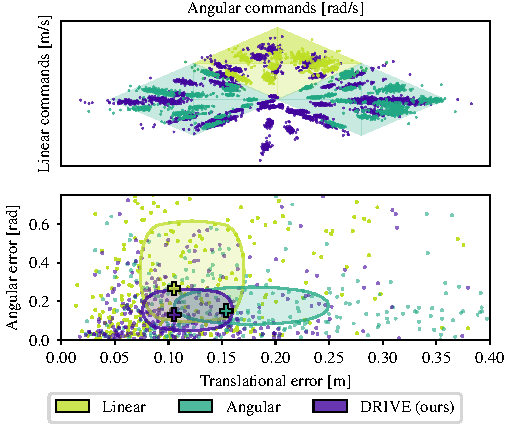
\includegraphics[width=0.7\textwidth]{./figures/sota_vs_doughnut_2_seconds_cg_v4.pdf}
		%\hfill
		\begin{minipage}[b]{.27\textwidth}%
			\captionsetup{justification=justified, name=Figure 2}
			\caption{
				Data-gathering protocol performance for the~\emph{HD2} on snow experiment.
				In yellow, we have the linear-focused method.
				In teal, we have the angular-focused method.
				In blue-violet is our DRIVE approach.
				The crosses and regions on the bottom subplot show the medians and interquartile ranges for translational and angular prediction errors.
			}
		\end{minipage}%
	\end{figure}
\end{block}





%----------------------------------------------------------------------------------------

\end{column} % End of the first column

\begin{column}{.03\textwidth}\end{column} % Empty spacer column
 
\begin{column}{.465\textwidth} % The second column

%----------------------------------------------------------------------------------------
%	New block
%----------------------------------------------------------------------------------------

\vspace{-12.5mm}
\begin{block}{Experimental Setup}
	\begin{itemize}
		\item Indoor tile, snow-covered terrain, gravel and surfaced ice.
		\item Three platforms: (1) the HD2 has a top speed of~\SI{1.2}{\meter / \second}; (2) Husky has a top speed of~\SI{1}{\meter / \second}; and (3) the the Warthog has top speed of~\SI{5}{\meter / \second}.    
		\item Over~\SI[detect-weight,mode=text]{7}{\kilo\meter} and~\SI[detect-weight=true,mode=text]{1.8}{\hour} of driving data.
	\end{itemize}
	
	\begin{figure}%
		\begin{minipage}[b]{.32\textwidth}%
			\captionsetup{justification=justified, name=Figure 3}
			\caption{
				Three different commercial platforms that were used for the experimental work:
				a \emph{Superdroid} HD2 (1), a \emph{Clearpath Robotics} Husky (2), and a \emph{Clearpath Robotics} Warthog mounted
				on wheels (3). 
				The platforms weigh~\SI{80}{\kilo\gram},~\SI{75}{\kilo\gram} and~\SI{470}{\kilo\gram}, respectively.
			}
		\end{minipage}%
		\hskip10mm
		%\hfill
		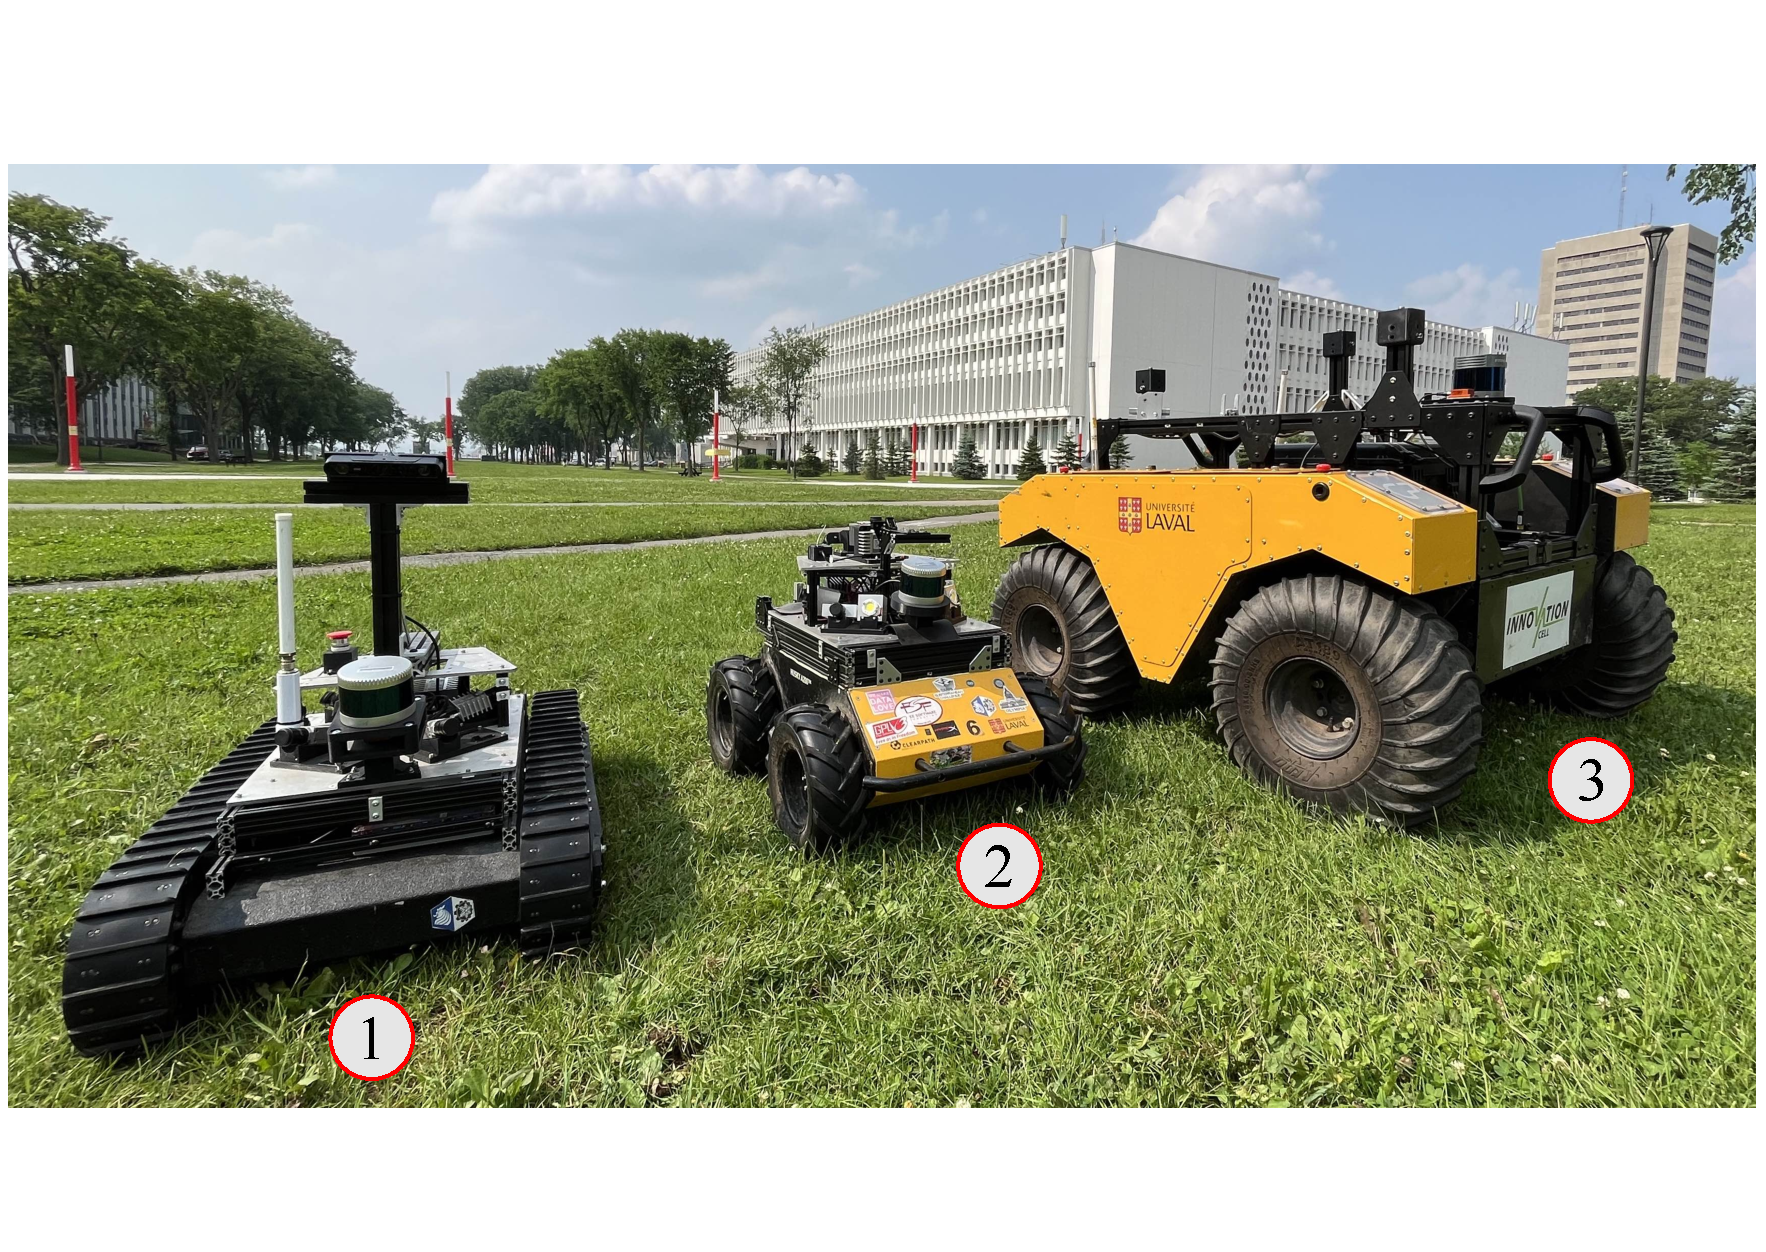
\includegraphics[width=0.63\textwidth]{./figures/norlab_robots_with_labels.pdf}
	\end{figure}
\end{block}


\begin{block}{Slip-based~\acf{BLR}}
	
	\begin{itemize}
		\item Additive slip model based on dynamics-aware basis functions~\cite{Seegmiller2014}.
		\item Leveraging~\acf{BLR} for learning motion parameters with minimal vehicle and terrain knowledge~\cite{McKinnon2019}.
		%\item Single-step slip learning.
		\item \ac{BLR} offers low computational complexity for fast learning.
		\item Each dimension of slip (longitudinal, lateral, angular) learned separately.
		\item First-order plus dead time transient response model for powertrain dynamics.
		\item Implimented and tested for~\acp{SSMR}.
	\end{itemize}
	
	\begin{figure}%
		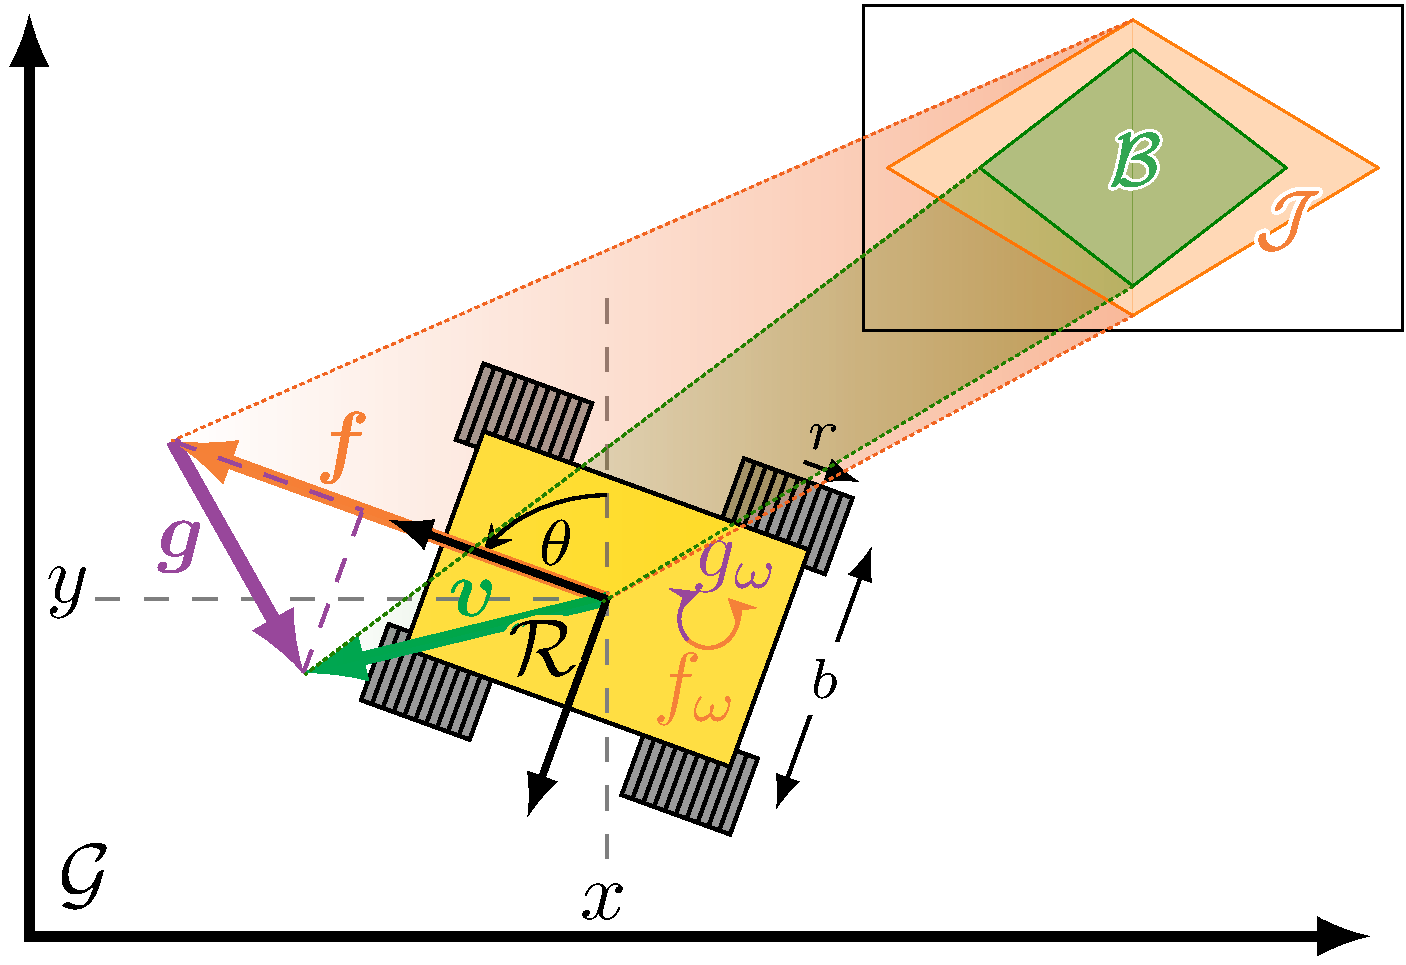
\includegraphics[width=0.6\textwidth]{./figures/Figure_2_final_no_margin-1.pdf}
		%\hfill
		\hskip1ex
		\begin{minipage}[b]{.35\textwidth}%
			\captionsetup{justification=justified, name=Figure 4}
			\caption{
				Top view drawing of a~\ac{SSMR}.
				In orange is the commanded body velocity~$\CMDBODYVEL$ and the resulting body velocity~$^{\robotf}\bm{v}$ is shown in green.
				The input-space~$\INPUTSPACE$ is shown in orange and the body velocity space~$\BODYVELSPACE$ is shown in green.
				The difference between commanded and resulting body velocity is represented as the slip velocity~$\SLIPBODYVEL$ in purple.
			}
		\end{minipage}%
	\end{figure}	
	\begin{itemize}
		\item Slip-\ac{BLR} outperforms the most similar model,which performs~\ac{BLR} on~\ac{UGV} actuator dynamics, by~\SI{6}{\%} in translation and~\SI{22}{\%} in rotation.
		\item Biggest improvement for Warthog on gravel with~\SI{23}{\%} in translation and~\SI{71}{\%} in rotation error. This is the highest top speed experiment.
		\item Model limit reached on surfaced ice, due to extreme slip and long transitory response.
		\item Powertrain model reduces prediction error for all models on each experiment.
	\end{itemize}
	\begin{figure}%
		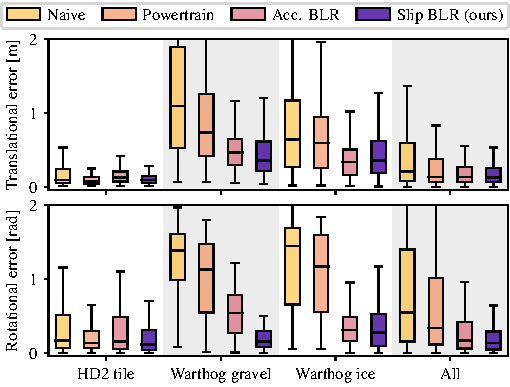
\includegraphics[width=0.73\textwidth]{./figures/prediction_errors_BLR_cg_v3.pdf}
		\hskip3mm
		%\hfill
		\begin{minipage}[b]{.23\textwidth}%
			\captionsetup{justification=justified, name=Figure 5}
			\caption{
				Translational and rotational prediction errors for all models studied in this work.
				In yellow is the manufactured-defined naive model, in orange is the powertrain-aware model, in red is the acceleration-based~\ac{BLR} model and in purple is our slip-based~\ac{BLR} model. 
				%Error medians are shown in black for all models.
			}
		\end{minipage}%
	\end{figure}
	
\end{block}

%----------------------------------------------------------------------------------------
%	ACKNOWLEDGEMENTS
%----------------------------------------------------------------------------------------


\begin{block}{Acknowledgments and References}
	\footnotesize%
	\noindent This research was supported by the Fonds de recherche du Québec – Nature et technologies (FRQNT) and by the Natural Sciences and Engineering Research Council of Canada (NSERC) through grant CRDPJ 527642-18 SNOW (Self-driving Navigation Optimized for Winter).
	%\vspace{-5mm}
	%\nocite{*} % Insert publications even if they are not cited in the poster
	\bibliographystyle{unsrt}%
	{\footnotesize\bibliography{biblio}}
	%\vspace{-3mm}
\end{block}



%----------------------------------------------------------------------------------------
%	CONTACT INFORMATION
%----------------------------------------------------------------------------------------
%
%\setbeamercolor{block title}{fg=black,bg=orange!70} % Change the block title color
%
%\begin{block}{Contact Information}
%
%\begin{itemize}
%\item Web: \href{http://www.university.edu/smithlab}{http://www.university.edu/smithlab}
%\item Email: \href{mailto:john@smith.com}{john@smith.com}
%\item Phone: +1 (000) 111 1111
%\end{itemize}
%
%\end{block}

%----------------------------------------------------------------------------------------

\end{column} % End of the second column

\begin{column}{.015\textwidth}\end{column} % Empty spacer column
\end{columns} % End of all the columns in the poster
%----------------------------------------------------------------------------------------
%	REFERENCES
%----------------------------------------------------------------------------------------
%
%\begin{block}{References}
%\vspace{-5mm}
%\nocite{*} % Insert publications even if they are not cited in the poster
%\bibliographystyle{unsrt}%
%{\small\bibliography{biblio}}
%\vspace{-3mm}
%\end{block}

\end{frame} % End of the enclosing frame

\end{document}
